\section{Architectural Design}
\subsection{overview}
The three-tier architecture model, which is the fundamental framework for the logical design model, segments an application's components into three tiers of services. These tiers do not necessarily correspond to physical locations on various computers on a network, but rather to logical layers of the application. How the pieces of an application are distributed in a physical topology can change, depending on the system requirements.
\newline
\newline
Other benefits (compared to single- or two-tier architecture) include:
\newline
 \textbf{Faster development:} Because each tier can be developed simultaneously by different teams, an organization can bring the application to market faster, and programmers can use the latest and best languages and tools for each tier.\newline\newline
 \textbf{Improved scalability :} Any tier can be scaled independently of the others as needed.\newline\newline
\textbf{Improved reliability:} An outage in one tier is less likely to impact the availability or performance of the other tiers.\newline\newline
\textbf{Improved security:} Because the presentation tier and data tier can't communicate directly, a well-designed application tier can function as a sort of internal firewall, preventing SQL injections and other malicious exploits.\newline\newline


\begin{figure}[H]
%\centering
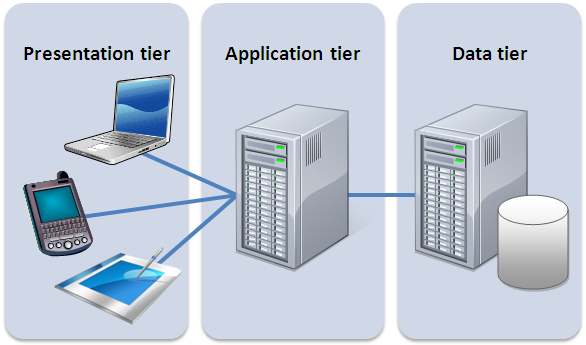
\includegraphics[width=1\textwidth]{figures/HighArchitecture.png}
\caption{\label{fig:student } Three tier Architecture }
\end{figure}

\subsection{High Level Components} 
\paragraph{}The architecture of the application is structured according to three logic layers:


 \textbf{ presentation tier}: or user services layer, gives a user access to the application. This layer presents data to the user and optionally permits data manipulation and data entry. The two main types of user interface for this layer are the traditional application and the Web-based application. Web-based applications now often contain most of the data manipulation features that traditional applications use. This is accomplished through use of Dynamic HTML and client-side data sources and data cursors.

 \textbf{The business tier}: or middle services layer, consists of business and data rules. Also referred to as the business logic tier, the middle tier is where COM+ developers can solve mission-critical business problems and achieve major productivity advantages. The components that make up this layer can exist on a server machine, to assist in resource sharing. These components can be used to enforce business rules, such as business algorithms and legal or governmental regulations, and data rules, which are designed to keep the data structures consistent within either specific or multiple databases. Because these middle-tier components are not tied to a specific client, they can be used by all applications and can be moved to different locations, as response time and other rules require. For example, simple edits can be placed on the client side to minimize network round-trips, or data rules can be placed in stored procedures.

\textbf{The data tier}: or data services layer, interacts with persistent data usually stored in a database or in permanent storage. This is the actual DBMS access layer. It can be accessed through the business services layer and on occasion by the user services layer. This layer consists of data access components (rather than raw DBMS connections) to aid in resource sharing and to allow clients to be configured without installing the DBMS libraries and ODBC drivers on each client.

\begin{figure}[H]
%\centering
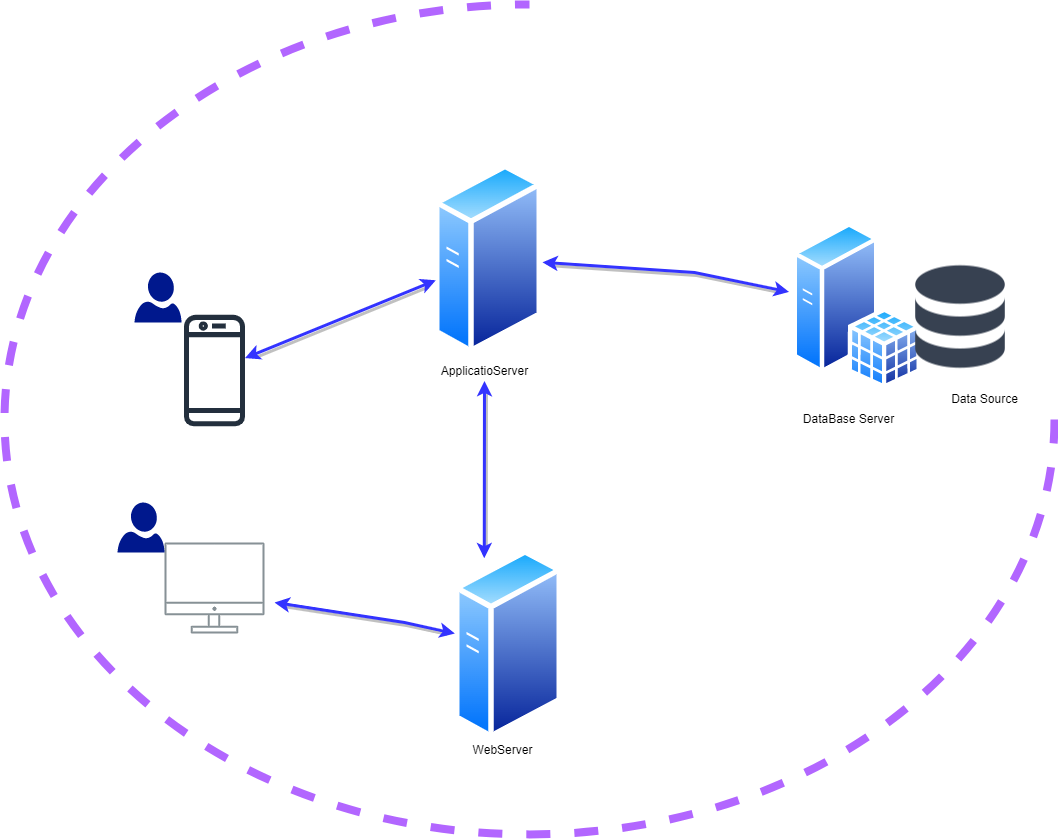
\includegraphics[width=1\textwidth]{figures/systemArchitecture.png}
\caption{\label{fig:student } the system Architecture }
\end{figure}

During an application's life cycle, the three-tier approach provides benefits such as re-usability, flexibility, manageability, maintainability, and solubility. You can share and reuse the components and services you create, and you can distribute them across a network of computers as needed. You can divide large and complex projects into simpler projects and assign them to different programmers or programming teams. You can also deploy components and services on a server to help keep up with changes, and you can redeploy them as growth of the application's user base, data, and transaction volume increases.
High Level Components
\clearpage

\subsection{Component View}

\begin{figure}[H]
%\centering

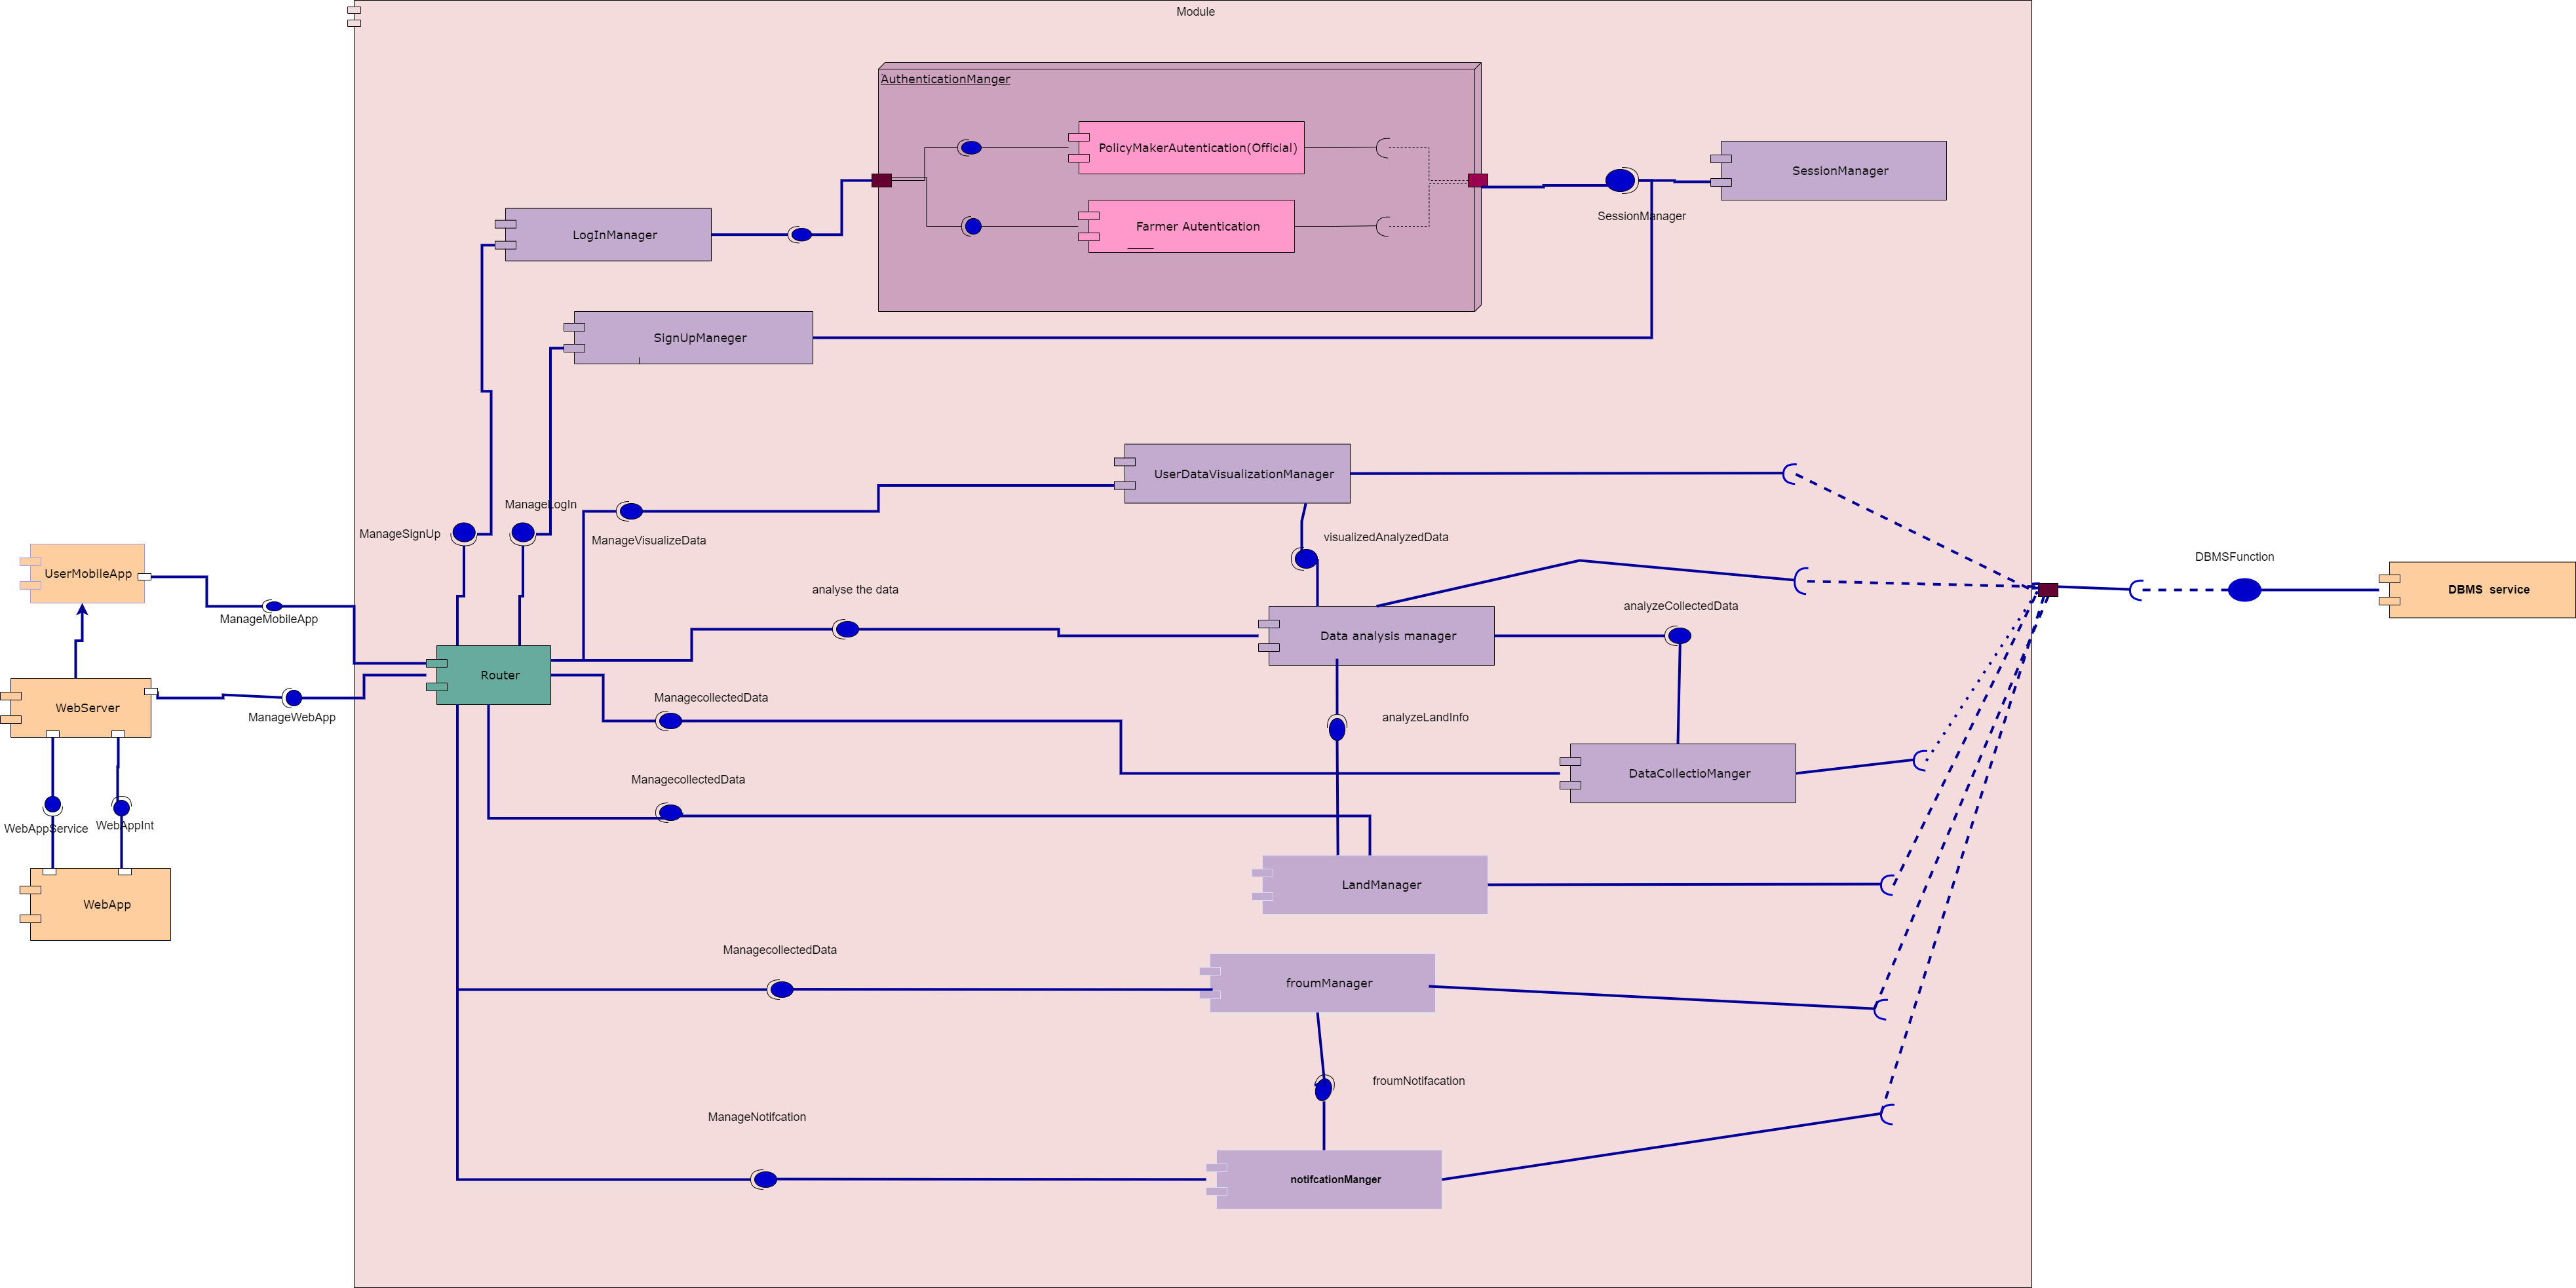
\includegraphics[angle=90,width=.6\textwidth]{figures/componenDiagramnew.png}
\caption{\label{fig:student } Component Diagram }
\end{figure}

\paragraph{} components’ functions contained in the ‘ApplicationServer’focusing on the representation of the internal structure of the application server, showing how its components interact. are described in the following:

\paragraph{NotificationManager:} it manages the notification which is used to send to users when its going to be close to be their turn and also their turn to enter the supermarket so it is connected to Estimator component.
\paragraph{DBMSManager:} this is the component that allows every other component in the system to interact with the database. The Interface provided by this component contains all useful methods to store, retrieve, update data into the database
from different actors. Every internal component of the application server uses some methods of its interface.
\paragraph{Router:} this component simply dispatches the requests and calls to methods from the users and the managers to the core of the application server. Every method is redirected to the proper component that can handle it. Also, responses and data sent back pass through this component to reach the applicant.
\paragraph{SignUpManager:} this component contains all the procedures to allow the farmer to register to \textbf{DREAM} expressing also to which service they want to register for.It has to interact with DBMS to store data about the registration and performing controls about the chosen username and password.
\paragraph{LoginManager:} it manages all the logic inherent to the authentication of the customers. It interacts with the DBMS to check that the authentication parameters match the stored ones.
\paragraph{Authentication component:}include two main sub component as follow:
\begin{itemize}
    \item \textbf{policymaker authentication (official):} this component check the credential and access level  with official organization and authorize them.
    \item \textbf{farmer authentication:} farmer authentication with saved data in database and check the access level.
    \item \textbf{session manager:} this component for authenticated user create the session and log the necessary information in database.also this delete the session after the user log out.
\end{itemize}

\paragraph{session manager:}this component for authenticated user create the session and log the necessary information in database.also this delete the session after the user log out.\newline
\paragraph{forum manager:}this component responsible for manage the forum such as create, delete topics and save the result on the database or manage the putting  comment or manage the question and answer and send the notification to related user.
\paragraph{land manager:}responsible to  related land function such as add new land,delete land or modify the production or fertilizer of land by given the location ID and save the changes in database.
\paragraph{data collection  manager:}This component responsible to  measure the environmental variable of farm land such as used water ,today weather and soil humidity and save in database.Also preparation data for analysing unit to have better performance.
\paragraph{data analysis manager: } this section analyze the function of the all farmer by environmental input such as used water,weather,soil humidity and out put is assess the farmer performance to show to the policymaker to encourage the best one and help to weak performance farmer
\paragraph{data visualization manager:}this section visualize the analyzed data about farmer progress(such as product and fertilizer recommendation) to show farmers to monitor the condition and improve the performance  
\subsection{Deployment View}
\begin{figure}[H]
%\centering
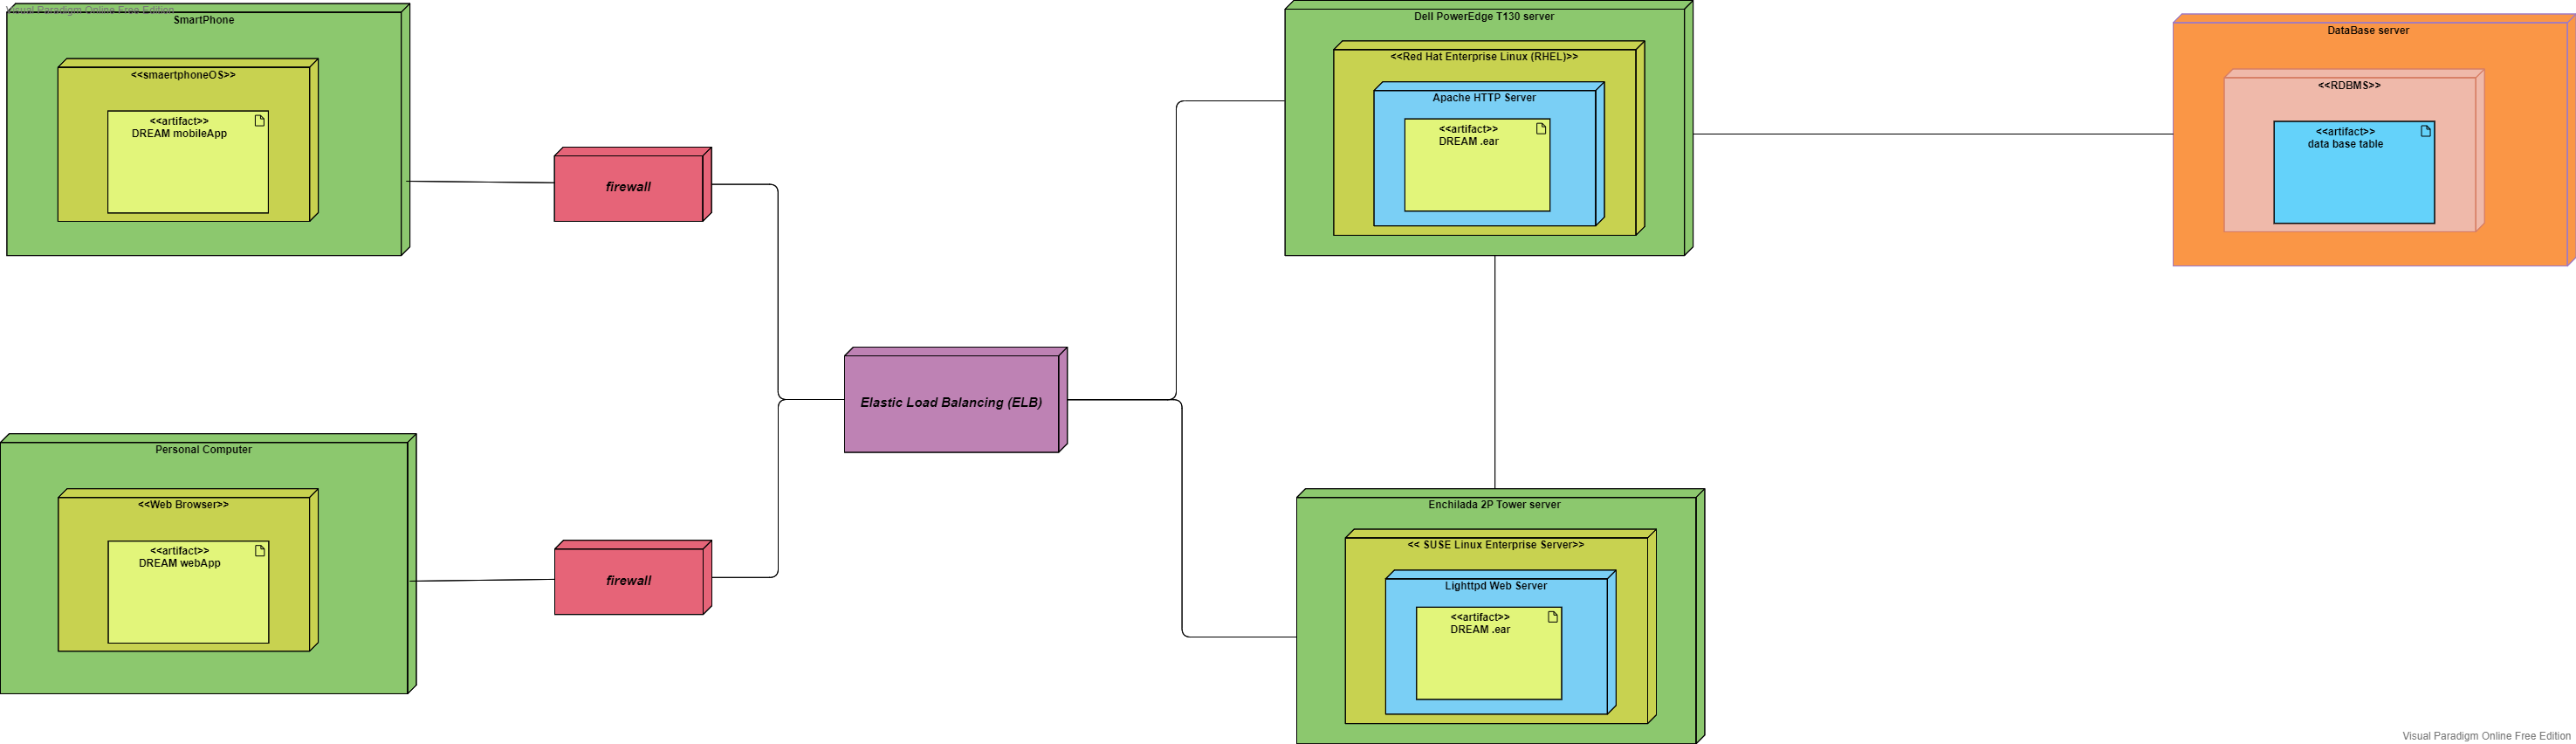
\includegraphics[width=1\textwidth]{figures/deploymentView.png}
\caption{\label{fig:student } deployment view }
\end{figure}
In the Deployment diagram in the figure are shown the most important components. A better explanation of these ones follows here:\\
\paragraph{Smartphone:} The farmers can use the smartphone to login and check the status of the their land or their progress on the other hand policy makers can monitor farmer performance by their smartphone .the information send  to the Application Server using HTTPS.
\paragraph{Computer:} another device to that farmer and policymakers can use to enter in\textbf{DREAM} is computer to have better experience to monitor of environmental situation and the progress.
\paragraph{Firewall:} Provides safety access to the internal network of the system as part of the safety of the system against external attacks.
\paragraph{Load balancer:} Distributes the workloads across multiple servers to increase capacity (concurrent
users) and reliability of applications trying to avoid the overload of any single server.
\paragraph{Web Server:} Receives contents and requests from clients through web app and sends data received, using Java RMI, to the Application Server for processing. Moreover, it is replicated to avoid a single point of failure and to guarantee a better performance.
\paragraph{Application/web Server:}Here we have the application logic, but not all because also the client has a part of this. The Application Server handles all the requests and provides the appropriate answers for all the offered services. It is directly addressed by the client app and , it is replicated just for having more accessibility an reliability.
\paragraph{Database Management System (DBMS):} is interface between the end user and the database, simultaneously managing the data, the database engine, and the database schema in order to facilitate the organization and manipulation of data.and we use  visualized and analyzed information by using  provided data from saved raw data in database.


\subsection{Run time view}
\subsubsection{Authenticate user}
\begin{figure}[H]
%\centering
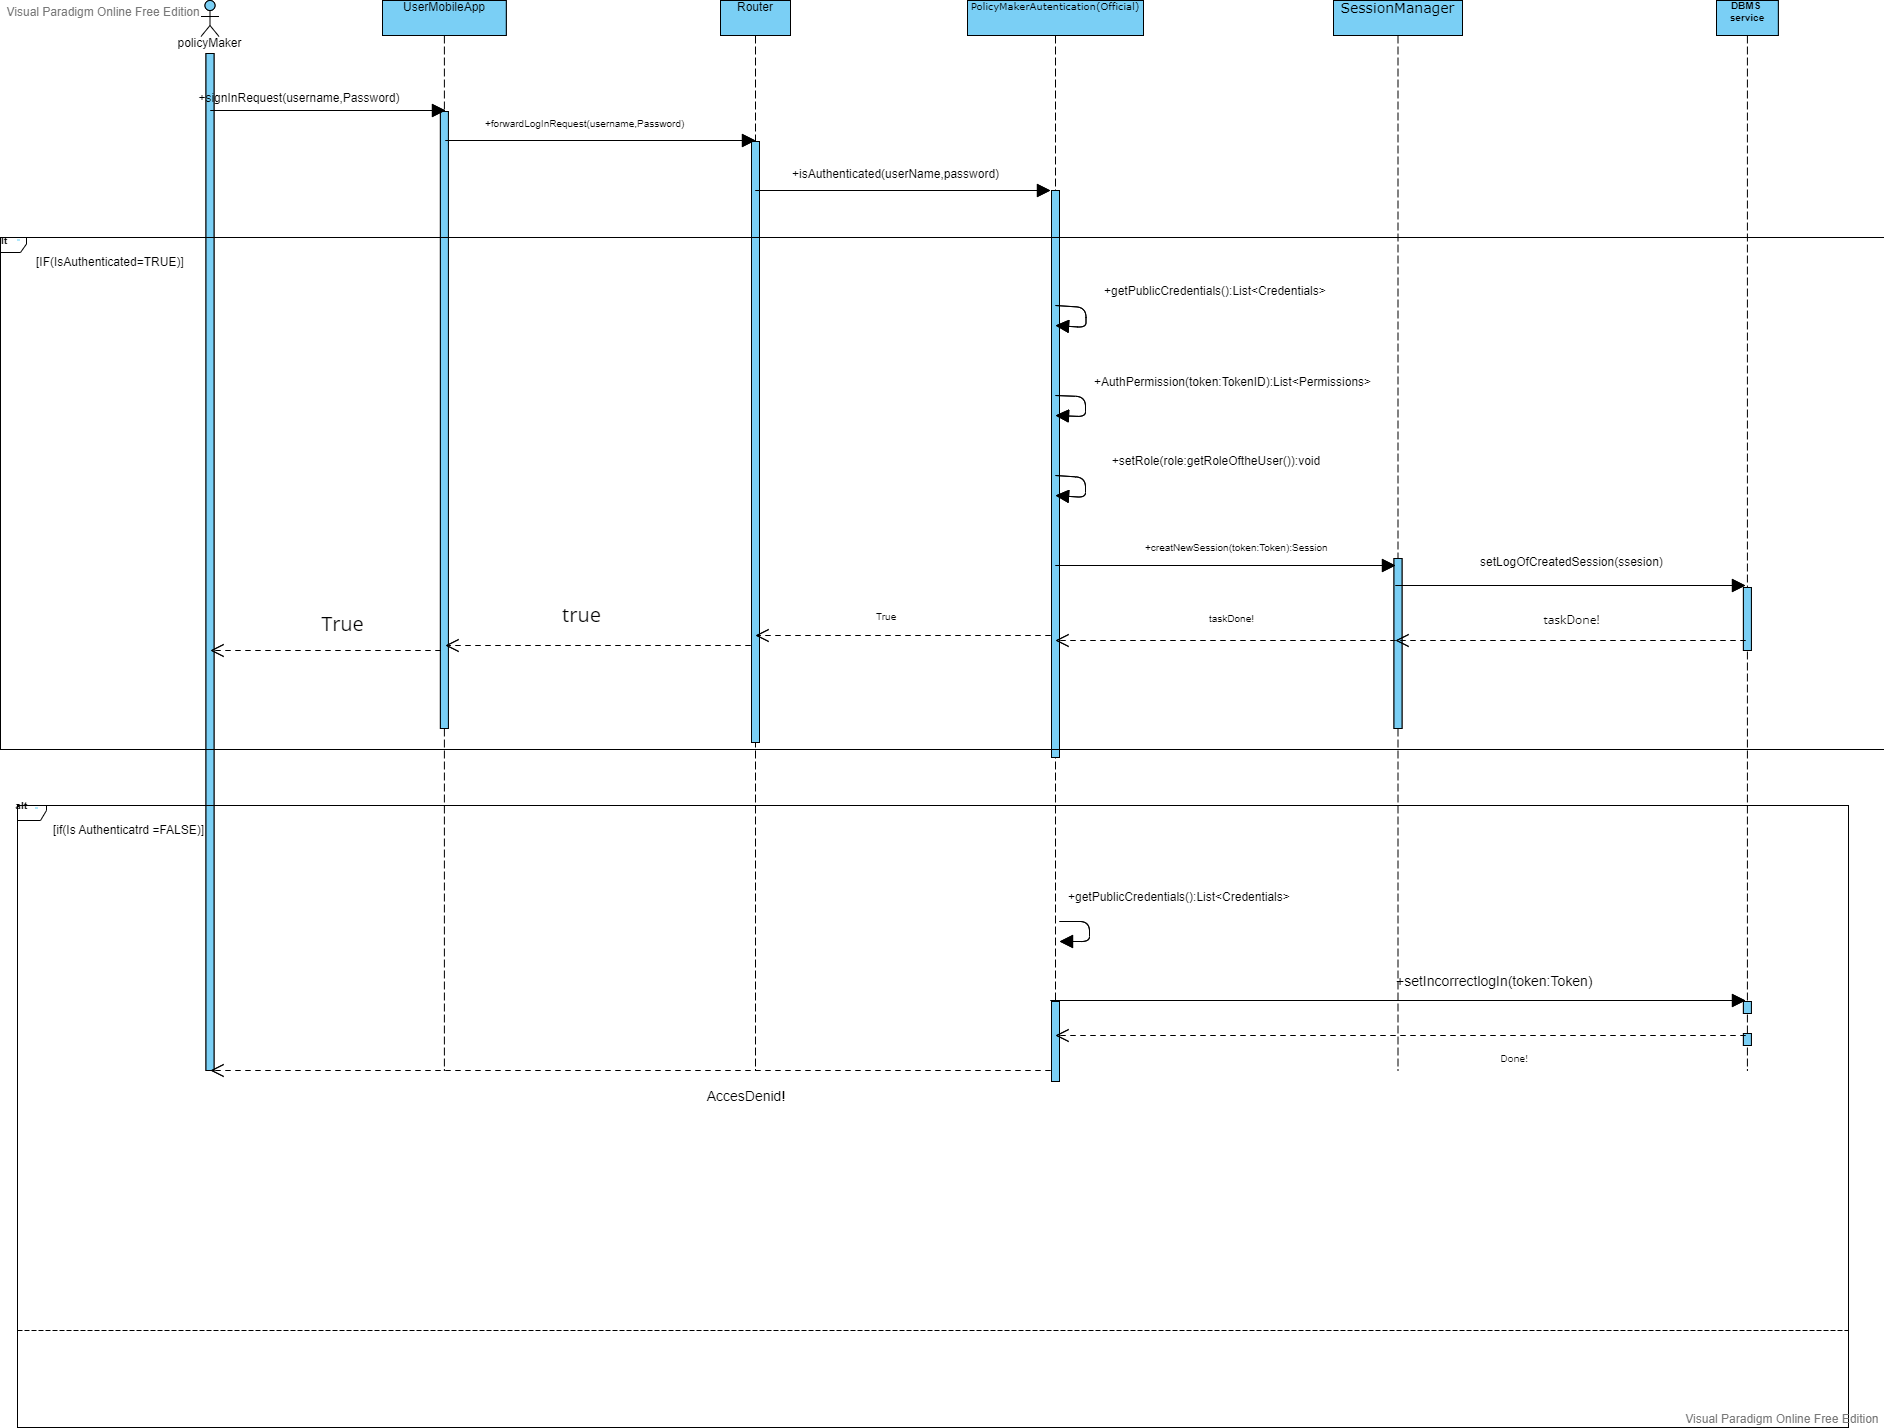
\includegraphics[width=1\textwidth]{figures/RunTimeSequenceDiagram-Page-1.png}
\end{figure}
In the sequence diagram shows how user is authenticated in our system.
first user request to log In in system by mobile application and with router this request is delivered to the login manager to validate the request and it to authentication component to export credential of the users and authorized them and dedicate the access by considering the their role in our system after the user data with role pass to the session manager to create new session and log necessary info in database .

\subsubsection{Analyse the Land Info}
\begin{figure}[H]
%\centering
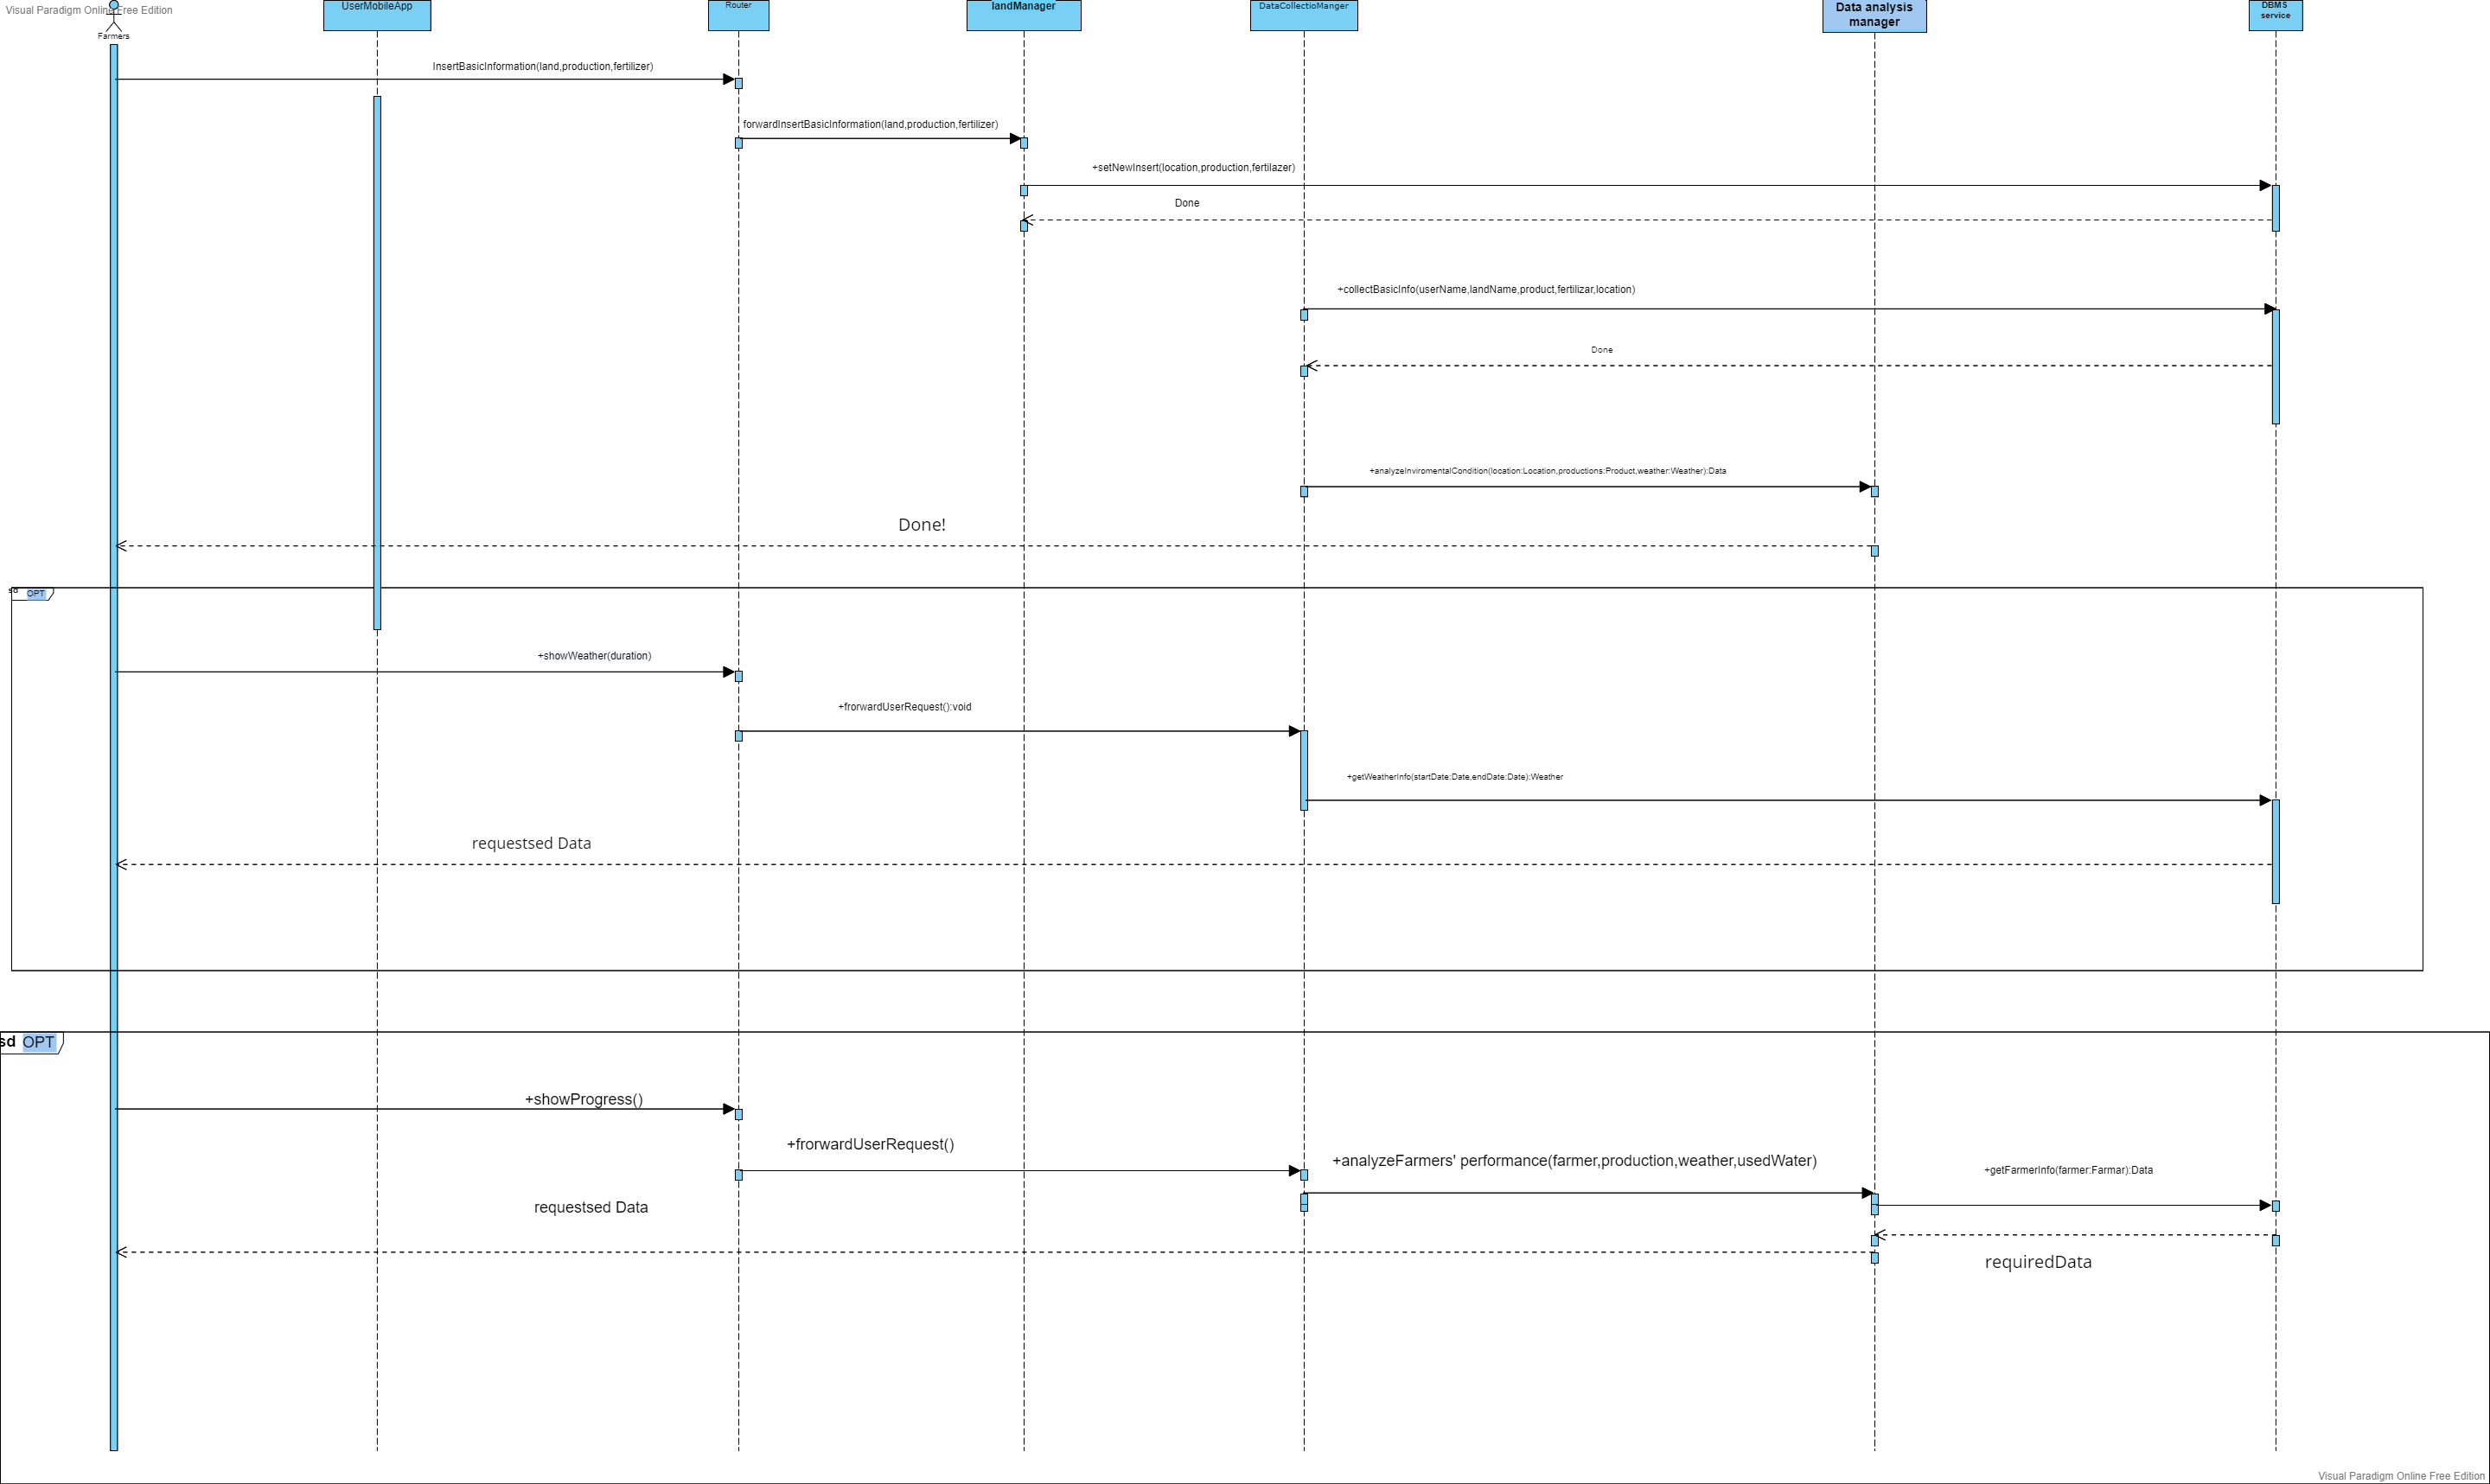
\includegraphics[width=1\textwidth]{figures/RunTimeSequenceDiagram-Page-2.png}
\end{figure}
In the sequence diagram shows how system make recommendation essential suggestion to farmer.
First farmer insert the her land information such as location and production  by the mobile application and router forward  this request to land manger that response for manage the affair of land and insert this information in database the collection section gather this info and measure other information such as weather condition and deliver this raw information to analyzer section  to process this info and suggest the best production and fertilizer can be used.\\
Also farmer can check the monitoring information such as his progress and or land weather  by mobile application and router forward the request to collection unit to gather appropriate info from database and show to the users
also analysing unit by provided info by collection unit can measure the farmer progress .

\subsubsection{Assess farmer progress }
\begin{figure}[H]
%\centering
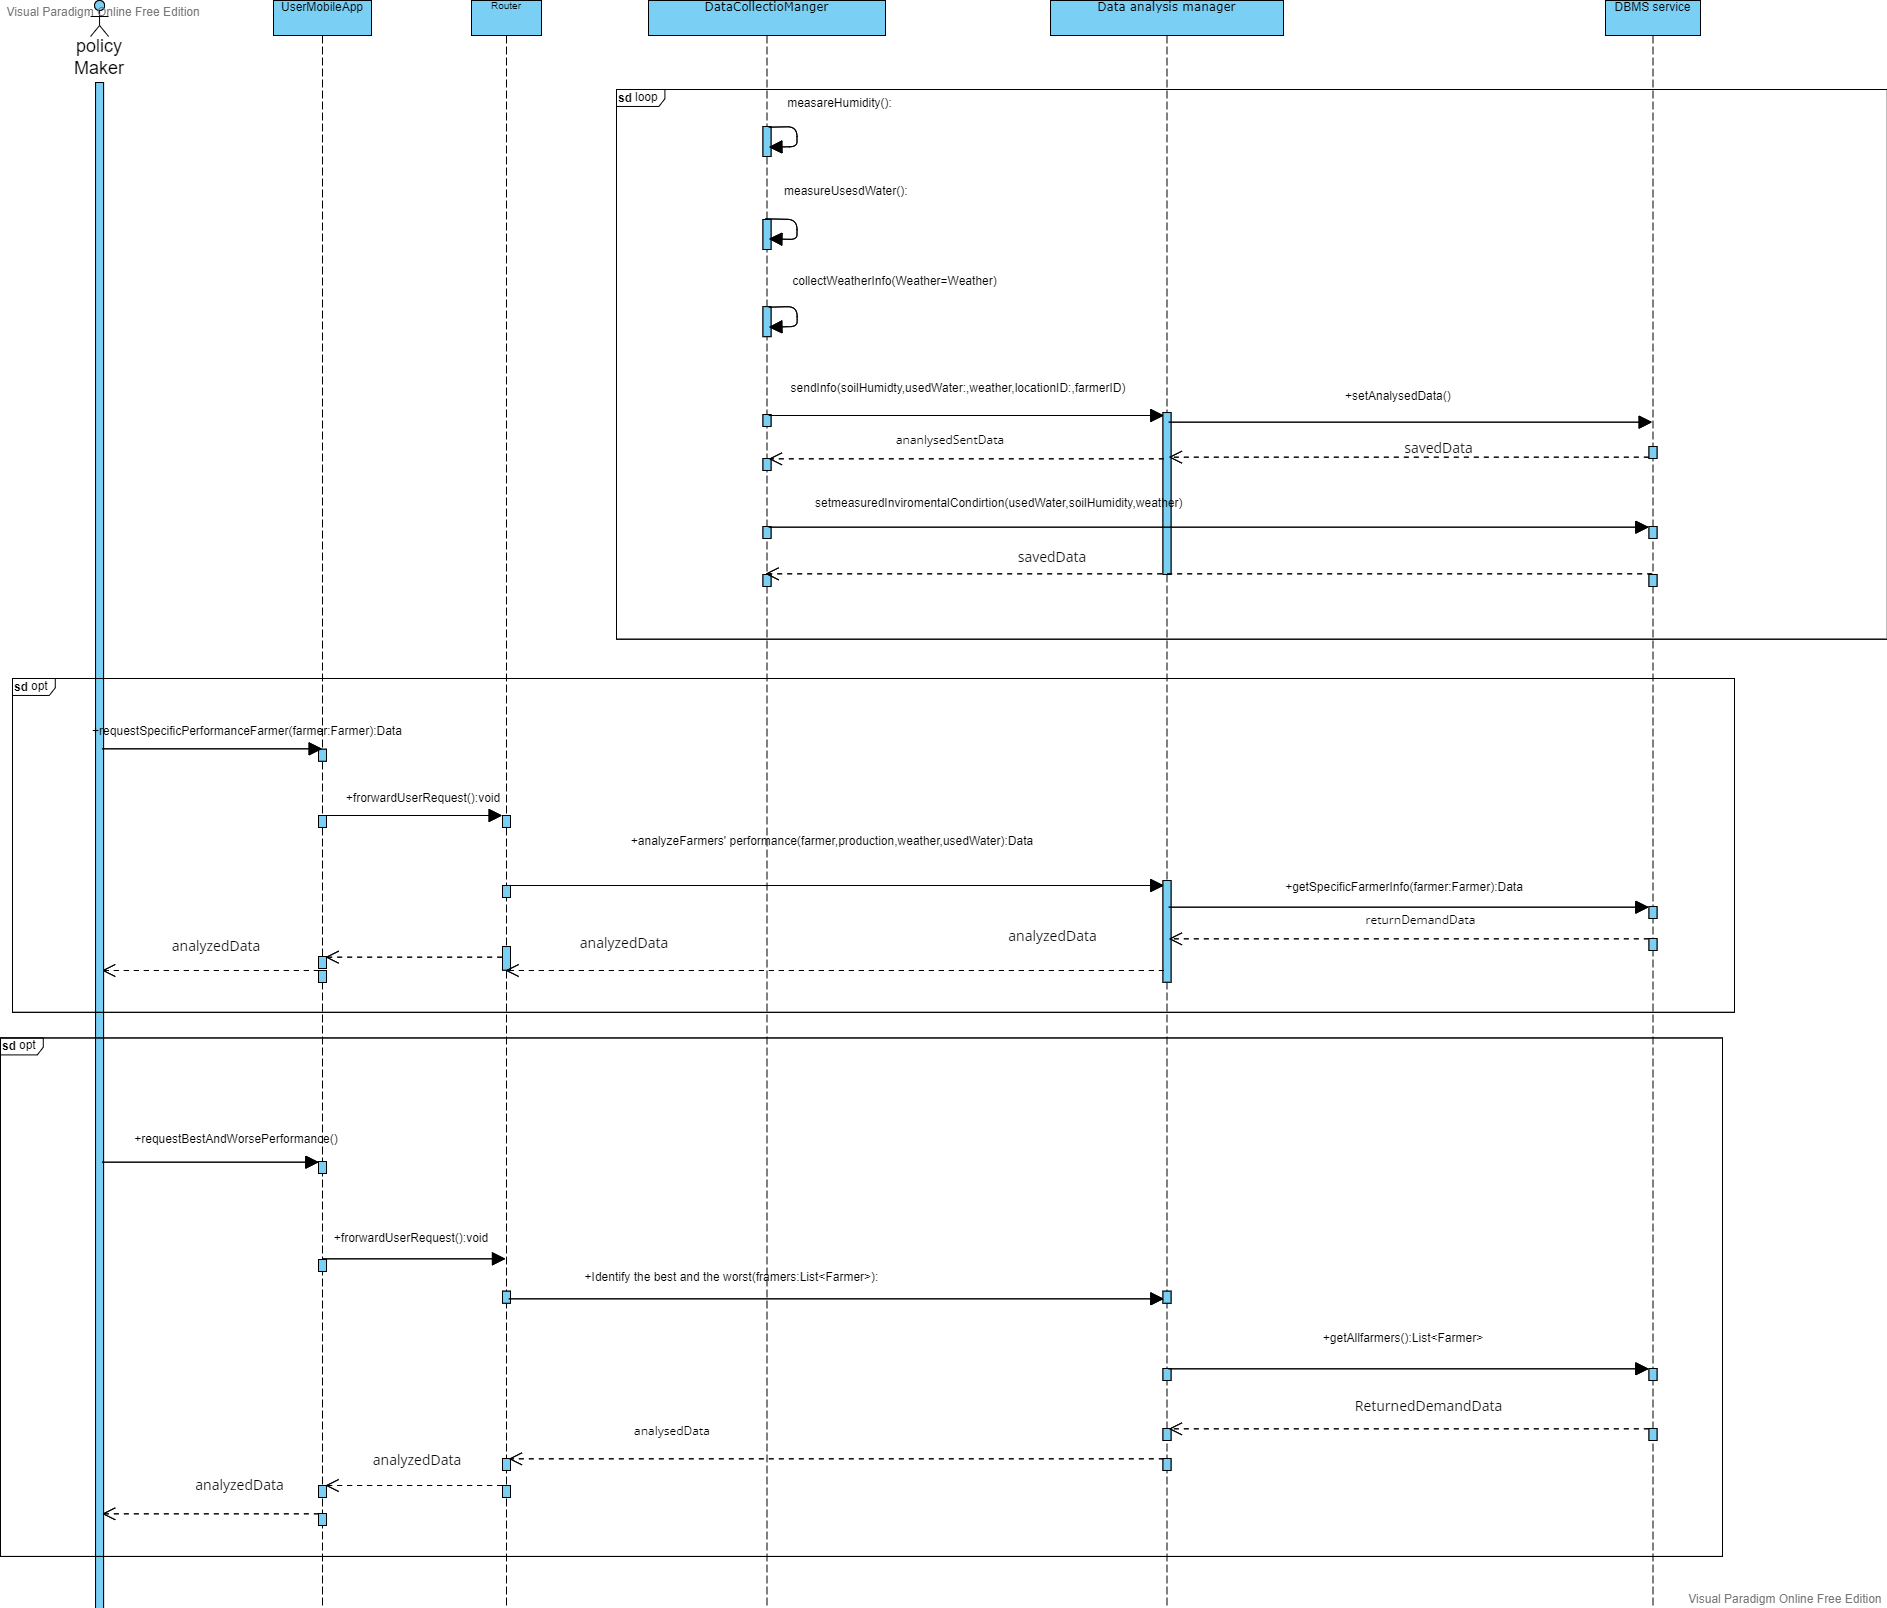
\includegraphics[width=1\textwidth]{figures/RunTimeSequenceDiagram-Page-3.png}
\end{figure}

In the sequence diagram shows how the policy maker assess  the farmer progress system continuously measure the the environmental variable by collection unit and get another information from database  and deliver this Information to analysis unit and after the saved this analysed data to database and then show to  policy maker if request to identify the best and worst farmer or and can request to see the specific farmer performance as the same way.
\subsubsection{forum activity}
\begin{figure}[H]
%\centering
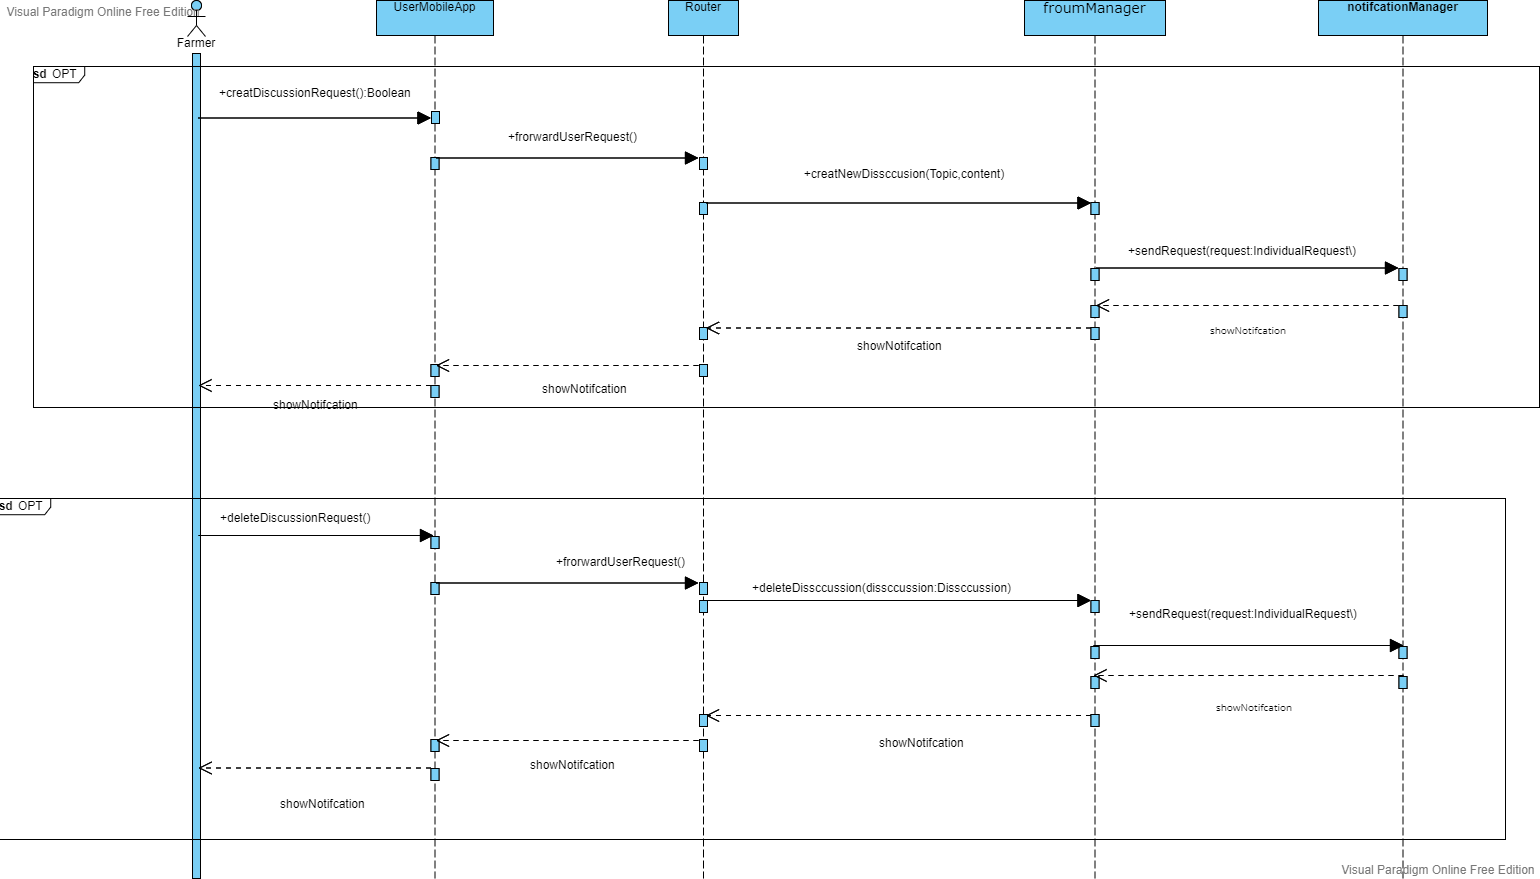
\includegraphics[width=1\textwidth]{figures/RunTimeSequenceDiagram-Page-4.png}
\end{figure}

In the sequence diagram shows how the farmer can have a activity in forum .
user can request to create the new topic router forward the request to forum manager and dedicate  a topic and content and save these formation in the  database also notify the user to these process done correctly.Also user can delete the past topic by his mobile application and router forward this request to forum manager and after this component save these change to database ,notify the user this process done correctly.    

\subsection{Component Interfaces}
In the next diagram are described the main methods which can be invoked on the interfaces and their interactions, referring to the most important processes reported in the run time view section.\newline
One aspect is fundamental to be pointed out: in general, methods written in the Component Interfaces diagram are not to be intended exactly as the methods that the developers will write, but they are a logical representation of what component interfaces have to offer. They will be adapted facing the various aspects that will come out during the implementation of the code


\begin{figure}[H]
%\centering
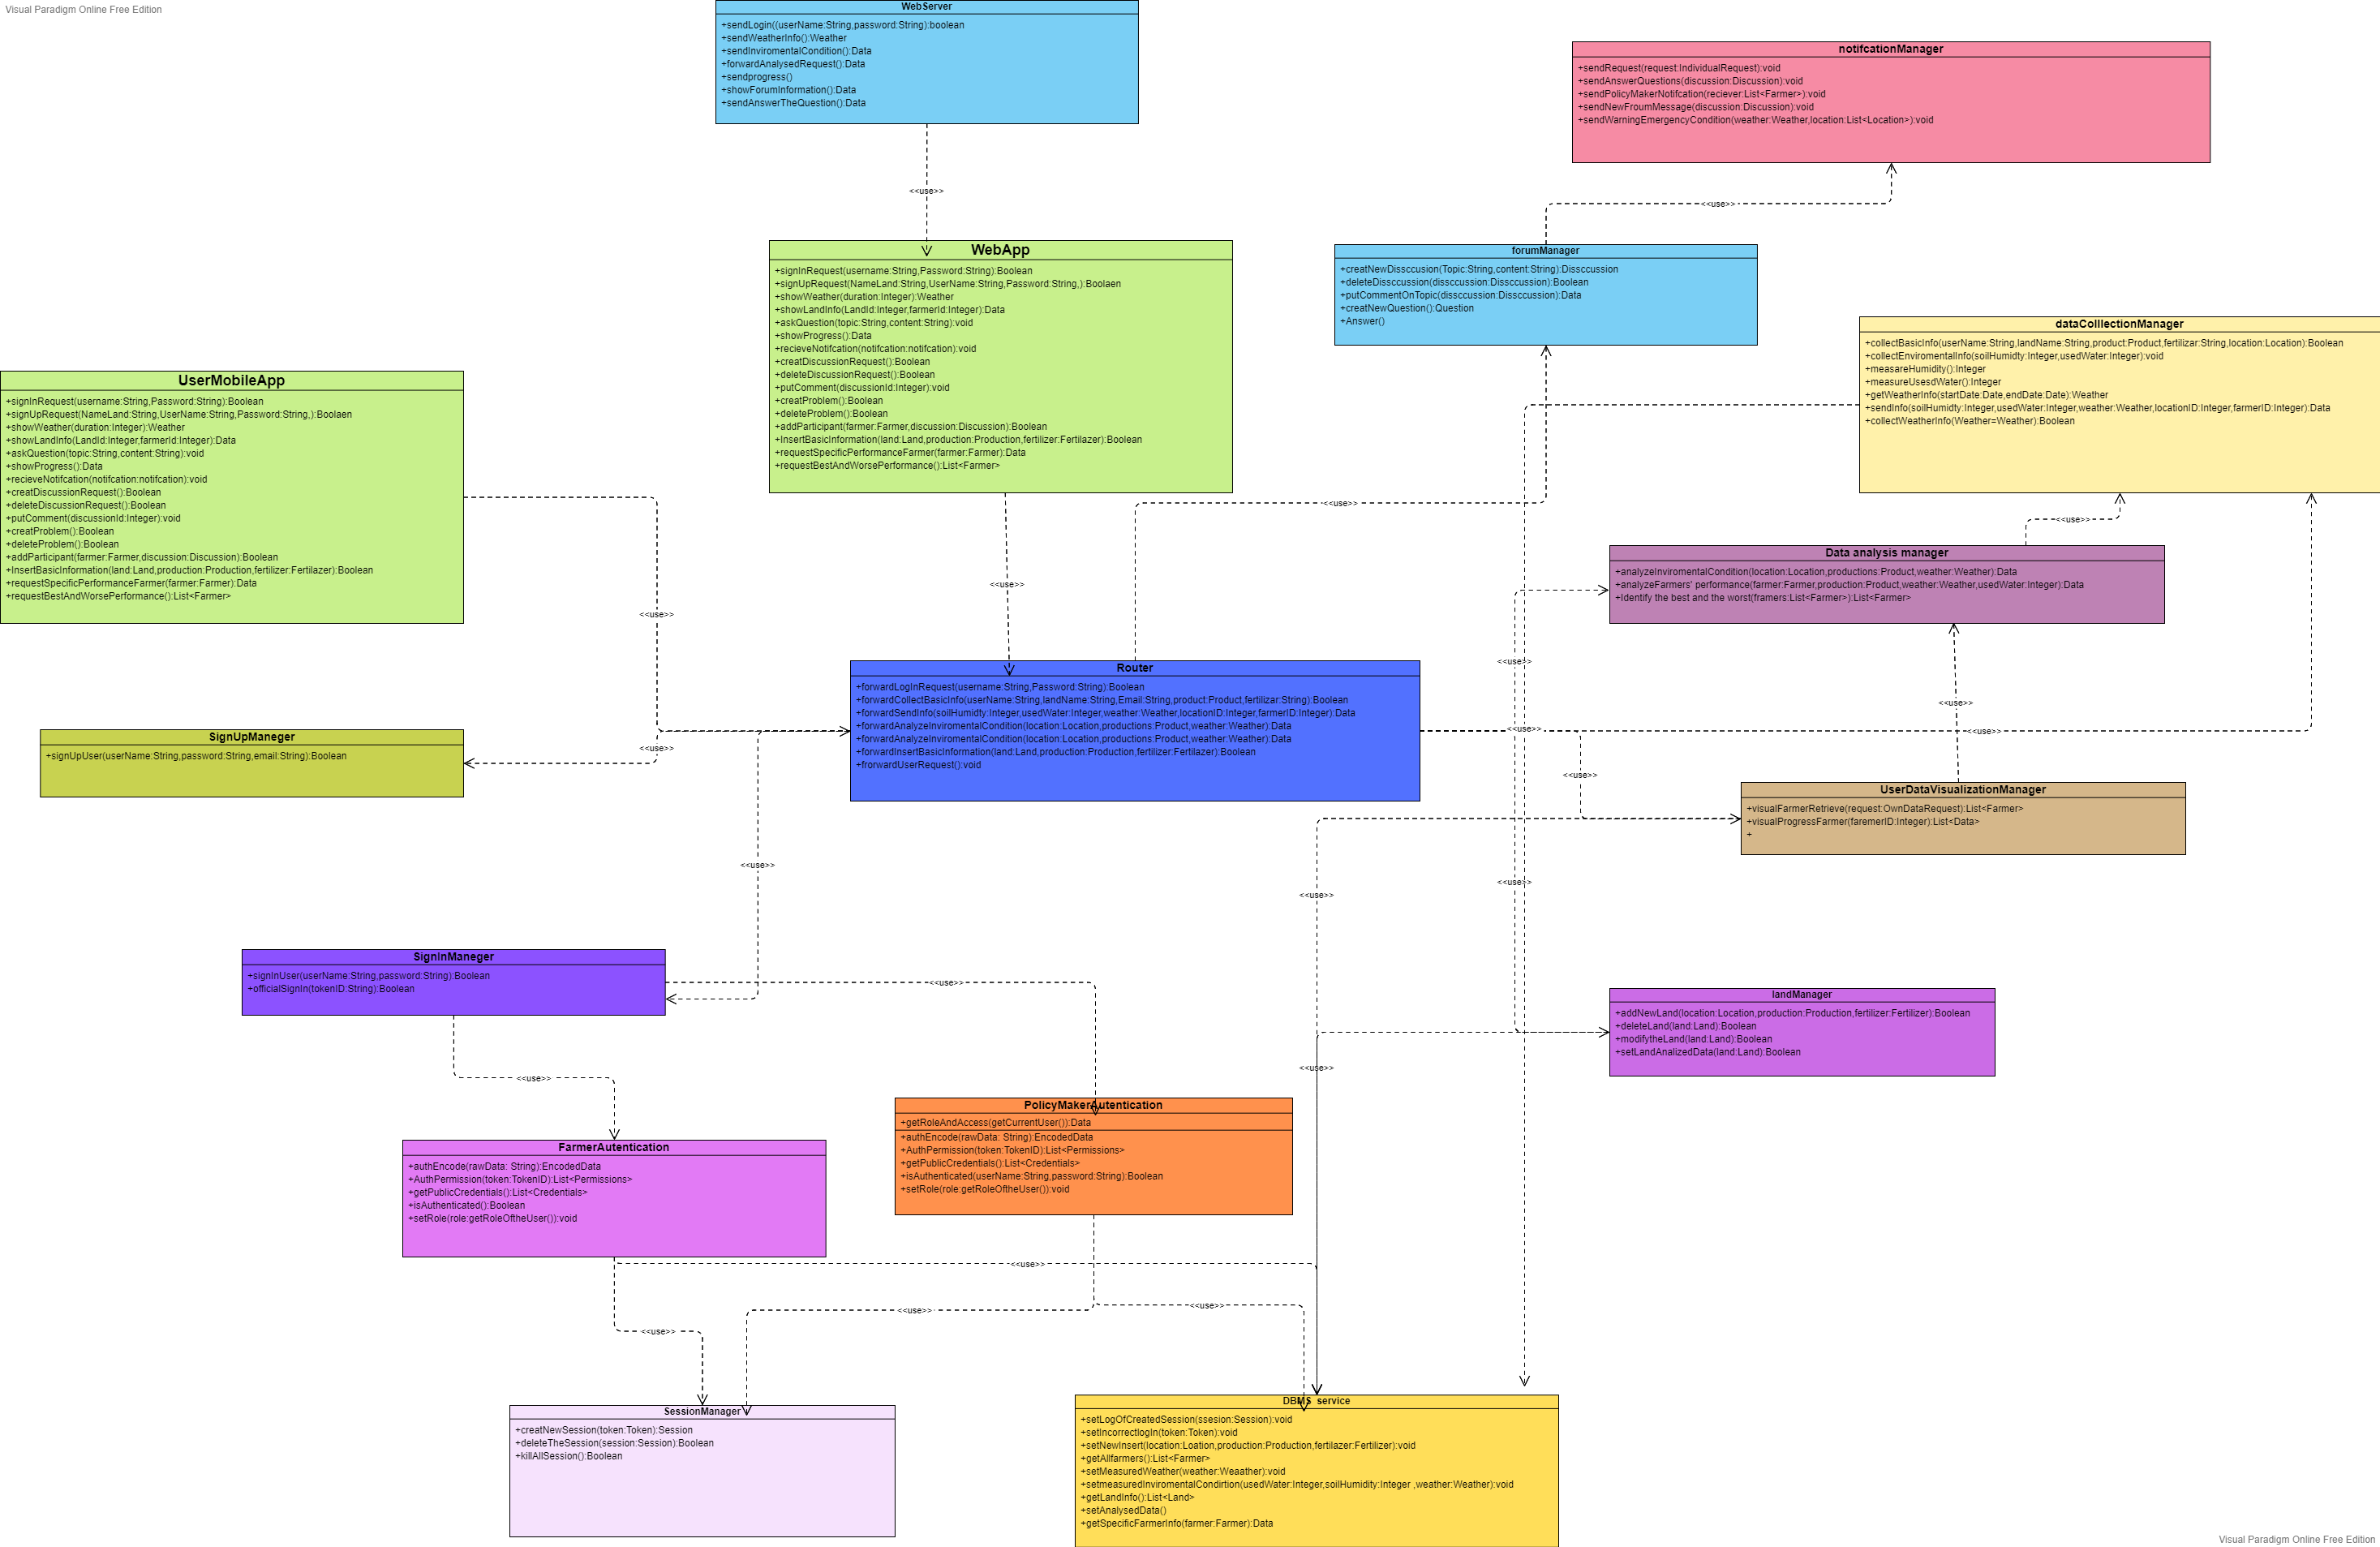
\includegraphics[angle= 90,width=1\textwidth]{figures/componentView.png}
\caption{\label{fig:student } component interface diagram}
\end{figure}

\subsection{Selected Architectural Style and Patterns}
Our system is based on a client/server architecture with three layers. Presentation, application and data access are physically separated. We choose this kind of architecture in order to have a modular system, also we use fat client to reduce the server load and smartphones nowadays are very powerful so, the costs of server will be less. Moreover we separated physically the database from the application server, to increase scalability and security, and it's also possible to use a distributed database. This choices promote a major decoupling of the system, increasing the reusability, scalability and  exibility.Furthermore, components in the application server have been thought to be cohesive and with low coupling among modules to make the system more comprehensible and modifiable.
The communication between the Mobile application and the Server will be done via
HTTP requests following REST principles. The communication between modules inside the application server and DB manager is RPC. When we use RPC, the programmer can use procedure call semantics and writing distributed applications is simplified.
because RPC hides all of the network code into stub functions.
\newline
In addition, we use some caches in the client side so we avoid some interactions between the client and server so we could reduce server loads. For example, in a short period of time users location do not change so, we could cache shops near the user for short amount of time and do not send requests to server.
We use JSON format for the communication data because, JSON uses less data overall,
so you reduce the cost and increase the parsing speed. Readable: The JSON structure
is straightforward and readable. You have an easier time mapping to domain objects,
no matter what programming language you're working with.
The model we choose for this project is Model View Controller (MVC). This model im-
proves the reusability and maintainability of code. One of the most important feature
of this design pattern is separation of concerns.\newline\newline
•\textbf{View:}  is that part of the application that represents the presentation of data.Views are created by the data collected from the model data. A view requests the model to give information so that it resents the output presentation to the user.\newline\newline
• \textbf{Controller} is that part of the application that handles the user interaction.\newline\newline
•\textbf{Model}  component stores data and its related logic. It represents data that is being transferred between controller components or any other related business logic.\newline\newline
\subsubsection{Other Design Decision}
In this section, we elaborate some decision we take.\newline\newline
\paragraph{ Flutter:} Flutter is a free, open-source mobile SDK that can be used to create native-looking Android and ioS apps from the same code base. Flutter helps
app developers build cross platform apps faster by using a single programming language, Dart, an object-oriented, class defined programming language. We chose to use this Framework in order to have a mobile app that works both with ioS and Android, with performances similar to the native development for each platform, but only having to write the code once. In Flutter, every piece of the user interface is a widget: like text, buttons, check boxes, images. There are also, "container widgets" that contain other widgets. Widgets can be stateless, which are immutable, or stateful, which have a mutable state and are used when we are describing a part of the user interface that can change dynamically.\\
Lastly we want to remember that Flutter is not the only framework that can be used to build cross-platform mobile apps, another option can be React Native, based on JavaScript. We decided to use Flutter because of it's advantages in comparison with React Native and other UI software development kit, which are: better performances and increasing popularity due to it's simplicity of develop.\\
\paragraph{ Golang:} Go is a statically typed, compiled programming language. Go has the same performance as C, but it is much easier to maintain than Java. Without the need for a virtual machine, Go boasts easier maintenance and no warming up period. These and many other characteristics are what make Golang stand out from its competitors.
\paragraph{Docker:} Containers work a little like VMs, but in a far more specific and
granular way. They isolate a single application and its dependencies|all of the
external software libraries the app requires to run|both from the underlying
operating system and from other containers. All of the containerized apps share
a single, common operating system (either Linux or Windows), but they are compartmentalized from one another and from the system at large.
The benefits of docker:
\begin{itemize}
    \item Docker enables more efficient use of system resources.
    \item Docker enables faster software delivery cycles.
    \item Docker enables application portability.
    \item Docker shines for micro services architecture
\end{itemize}

\clearpage